\section{Marco Teórico}

\subsection{Microcontrolador ATmega328P}

\subsection{Registros de propósito general}

\subsection{Entradas y Salidas Digitales}
\begin{itemize}
    \item Concepto de GPIO.
    \item Uso de pulsadores como entradas digitales (debouncing si es necesario).
    \item Uso de LEDs como indicadores de estado.
\end{itemize}

\subsection{Stack Pointer}
El stack pointer es una herramienta utilizada dentro de la programación del microcontrolador. El stack pointer es un no es nada más que un puntero interno del microcontrolador (similar a X, Y o Z) el cual tiene una serie de operaciones asignadas, y un comportamiento específico. El stack pointer se inicializa al final de la memoria RAM, alejado de todo para intentar no molestar al resto. Véase anexo \ref{anexo:Stack_Pointer}

Allí el stack pointer queda como la cima de la pila y, en AVR, la pila crece hacia direcciones más bajas: un PUSH decrementa primero el SP y luego escribe el dato; un POP lee el dato y después incrementa el SP. Las llamadas a subrutinas (CALL/RCALL) empujan automáticamente la dirección de retorno (PC) a la pila y RET la recupera. En una interrupción, el hardware apila el PC y el registro de estado SREG; RETI los restaura. Además, las rutinas suelen guardar con PUSH los registros que van a usar y devolverlos con POP al salir para no corromper el contexto.

Instrucciones como call, rcall, o las interrupciones dependen de la inicialización previa del Stack Pointer, para poder funcionar de manera adecuada, ya que el Stack Pointer es el que se encarga de guardar las direcciones de memoria a las cuales estas instrucciones deben retornar luego de terminar la ejecución, de no estar inicializado el Stack Pointer, el programa no sabría a donde volver luego de una interrupción, muy probablemente yendo a una dirección del programa aleatoria y rompiendo el flujo del codigo. Véase anexo 

\subsection{Delay activo}
Un delay activo es una pieza de código que toma en cuenta el la velocidad de ejecución del microcontrolador, para ejecutar un número de instrucciones (inútiles) concreto, representando un pasaje de tiempo específico, para luego retornar al flujo del programa. Son fáciles de usar, pero no es recomendable abusard de ellas debido a ineficiencias energéticas, y que el programa se mantiene ocupado la mayor parte del tiempo en el temporizador, en lugar de poder dedicarse a hacer otras tareas. Véase anexo \ref{anexo:Delay_Activo}, allí se encuentra un ejemplo de un delay activo.

\subsection{Timers}
Timer 0 y 2 son de 8 bits. Timer 1 es de 16 bits, por lo que puede contar intervalos más largos y con mejor resolución. Cada timer toma su reloj de la CPU y lo divide con un prescaler \(N\). El tiempo de cada tic es:

\[
t_{\text{tick}}=\frac{N}{f_{\text{CPU}}}.
\]

La ecuación para calcular el tiempo de desborde es:

\[
    \frac{(2^{k} - C_{\text{inicio}})\cdot \text{Prescaler}}{f_{\text{contador}}} = t_{\text{deseado}}
\]


Esta ecuación determina el tiempo que le tomaría al contador hacer un desbordamiento (overflow) en base a la frecuencia a la cantidad de bits del contador (k), la frecuencia de trabajo del microcontrolador, el tiempo o conteo con el que se inicie el contador, y el prescaler con el que esté configurado. En el anexo \ref{anexo:Configuracion_Timer_1} podrá encontrar un procedimiento detallado de como configurar el Timer 1.

\subsection{Interrupciones externas}

   \begin{figure}[H]
    \centering
    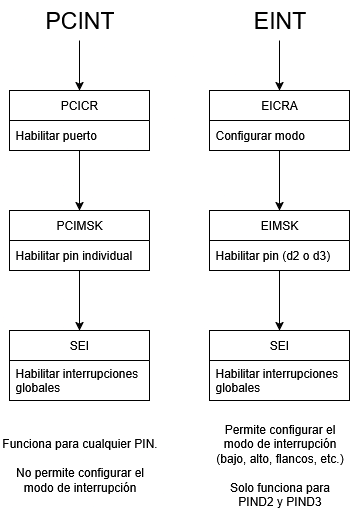
\includegraphics[width=0.7\linewidth]{./Anexos/Marco Teorico/External Interrupts/Interrupt diagram.png}
    \caption{Flujo de configuración de interrupciones exeternas. Fuente: Elaboración própia.}
    \label{fig:InterruptDiagram}
    \end{figure}


    \subsubsection{EINT}


    \subsubsection{PCINT}

\subsection{SRAM}

% Anexo: Como reservar sram
%       Como escribir sram
%       Como leer sram

Usando dseg se puede reservar espacio en memoria la SRAM para utilizarlo luego. Posteriormete con ``variable'' podremos leer o escribir el valor guardado con ``lds'' o ``sts'' respectivamente. O incluse se podría utilizar un puntero (X, Y, Z) para acceder a un lugar en memoria de manera iterativa donde quisieramos guardar múltiples valores subsecuentes (como un arreglo). 

Nota: Existen 2kb de memoria RAM, el stack pointer vive dentro de la RAM así que uno debe ser precabido con el uso excesivo de este recurso.

\subsection{FLASH}

Utilizando .cseg y una dirección segura como 0x300 para guardar datos, se puede utilizar la misma memoria FLASH para guardar datos constantes como LUTs, fotogramas, cadenas de texto, etc. Estos datos no pueden ser modificados, pero existen 32kb de espacio en memoria FLASH para guardar información, por lo que es menos limitante que la SRAM (2kb).

Para acceder a datos guardados en program memoria del programa (FLASH) se puede hacer haciendo uso del puntero Z y la instrucción ``lpm''. En ``Z'' Se carga la dirección a Z cargando las partes bajas y altas de la dirección a ZL y ZH respectivamente. En los AVR  ``clásicos'' (como el ATmega328P), las etiquetas en memoria de programa (.cseg) están en direcciones de palabra (cada instrucción ocupa 16 bits), pero la instrucción LPM usa una dirección en bytes en el registro Z. Por eso se hace $<$$<$ 1 (multiplicar por 2): convierte la dirección en palabras de la etiqueta a dirección en bytes para LPM. Y ``Z+'' indica que luego de realizar lpm, se incremente en 1 el puntero ``Z''. Véase anexo \ref{anexo:FLASH}

\subsection{Bit masks}
Una máscara es un número binario, pero en una máscara lo que nos importa es la posición de los unos y ceros en lugar del valor mismo que representan. Un mismo valor binario puede representar un número o una máscara, solo depende de como lo mires.  

``ldi r16, 0b00001010 out PORTB, r16'' carga una máscara de bits al puerto B para encender los pines 1 y 3, y apagar el resto, pero también se puede ver como que se está cargado el número 10 al puerto B (``ldi r16, 10 out PORTB, r16'')

Saber operar con máscras se vuelve útil cuando, por ejemplo, se busca afectar solo uno o varios bits en específico de un registro. En ese caso,  Lo que se hace primero es leer el registro, luego se realizar una operación lógica con la máscara que representa los bits que se quieren afectar, y por último se carga la máscara modificada al registro. Este tipo de operaciones se vuelve muy común cuando se trabajan con matrices LED, donde es muy común tener que mezclar puertos entre filas y columnas. Véase anexo \ref{anexo:Bit_Masks}


\subsection{LUT}
Para trabajar de manera ordenada en el desorden. Convierte al dolor de cabeza que son los puertos, en simples operaciones de lectura de FLASH, y modificación de punteros. Véase anexo \ref{anexo:Look_Up_Table}

\begin{figure}[H]
  \centering
  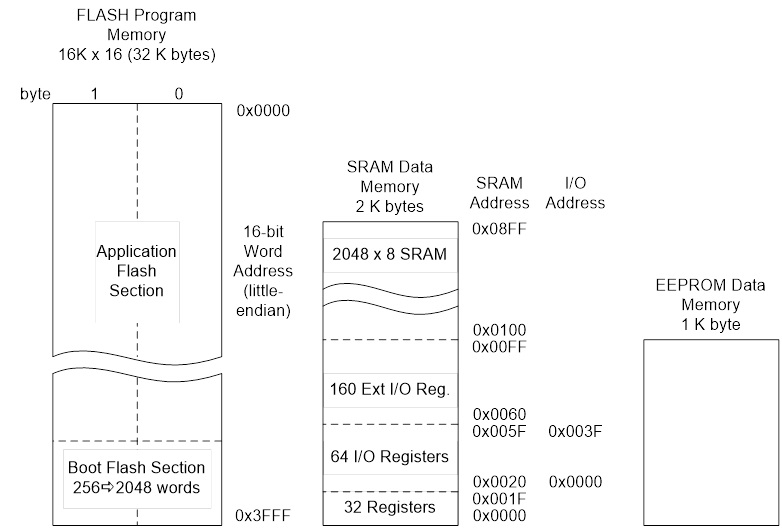
\includegraphics[width=\linewidth]{./Anexos/Memory Map.jpg}
  \caption{Mapa de memoria y espacios de direcciones en AVR de 8 bits. Fuente: \cite{arxterra_avr_addressing_modes}.}
  \label{fig:avr-memory-map}
\end{figure}

\subsection{USART asíncrono}

\subsection{Ring Buffer}

\subsection{USART asíncrono con Ring Buffer}

\subsection{Automatización y Máquinas de Estado}

\subsection{Kit FischerTechnik}

\begin{itemize}
    \item Principios básicos de una cinta transportadora en automatización.
    \item Funcionamiento de un actuador lineal/solenoide como punzón.
    \item Diferentes modos de operación según carga (ligera, media, pesada).
\end{itemize}


\subsection{Conversión Digital-Analógica (DAC R-2R)}
Un DAC (Digital to Analog Converter) es un dispositivo o técnica que permite transformar valores digitales (códigos binarios) en señales analógicas (tensiones o corrientes continuas y variables en el tiempo). Su importancia radica en que la mayoría de los sistemas electrónicos trabajan de manera digital, pero el mundo físico es analógico: audio, imágenes, señales de control de motores, etc.

El arreglo R-2R es una red de resistencias que se usa mucho para construir DACs simples y económicos. Se compone unicamente de dos valores de resistencias: una de valor R y otra de valor 2R, que se repiten en forma de escalera.

Cada bit del número digital controla un pin de los puertos del microcontrolador que conecta la red a una referencia de tensión (Vref) o a tierra. Gracias a la proporción entre Ry 2R, la red genera tenciones que corresponden al valor binario aplicado.

Una Look-up Table (LUT) es básicamente una tabla de valores precargada en la memoria que representa una señal digitalizada (por ejemplo, una onda seno). En lugar de calcular cada valor de la función en tiempo real, el monitor solo ``lee'' la tabla en orden y envía los valores a un puerto o a un DAC.Cuando esos valores se aplican de manera periódica y con la velocidad adecuada, en la salida se reconstruye una señal analógica periodica.
    

\subsection{Matriz de LEDs}
Modelo 1088AS: matriz 8×8 de cátodo/anodo multiplexado, apta para control por filas y columnas. La disposición exacta de pines se encuentra en el anexo \ref{anexo:Matriz_de_LEDs_1088AS}. Para encender un LED específico, se aplica nivel 0 a la fila correspondiente y nivel 1 a la columna correspondiente.




\subsection{Plotter y Control de Movimiento}
Un plotter es un sistema de trazado que posiciona un útil (lápiz/solenoide) en X–Y para dibujar o marcar piezas. En ingeniería se usa para prototipado, plantillas y pruebas de control de movimiento.

El movimiento puede lograrse con motores paso a paso o con motores conmutados mediante relés/MOSFETs. En el primer caso se controlan pasos y dirección; en el segundo, sentido y velocidad (opcionalmente con PWM). El útil sube y baja con un solenoide controlado también por una salida digital.

Este plotter ya tiene un Arduino conectado al \texttt{PORTD}. Cada bit de \texttt{PORTD} activa una acción: arriba, abajo, izquierda, derecha, subir solenoide, bajar solenoide. La tabla de comandos está en el anexo \ref{anexo:Comandos_Plotter}.




